\documentclass[11pt]{article}

% margins
\usepackage[margin=0.75in]{geometry}

% figures
\usepackage{graphicx}

% font
\usepackage{mathpazo}

\usepackage{helvet}

% coloring
\usepackage{color}
\definecolor{mygray}{gray}{0.5}

% footer
\usepackage{fancyhdr}
\pagestyle{fancy}
\fancyfoot[LO,LE]{\footnotesize \sffamily \color{mygray} M.\ Zingale---Notes on Advection}
\fancyfoot[RO,RE]{\footnotesize \sffamily \color{mygray} (\today)}
\fancyfoot[CO,CE]{\thepage}
\fancyhead{}
\renewcommand{\headrulewidth}{0.0pt}
\renewcommand{\footrulewidth}{0.0pt}

% captions
\usepackage{caption}
\renewcommand{\captionfont}{\footnotesize}
\renewcommand{\captionlabelfont}{\footnotesize}
\setlength{\captionmargin}{5em}


\usepackage{sectsty}
\allsectionsfont{\sffamily}

\usepackage{amsmath}

\begin{document}

\begin{center}
{\LARGE \textsf{\textbf{
Notes on Advection}}
}
\end{center}

\begin{quote}
\noindent {\em These notes introduce the basic
numerical methods for dealing with advection, using finite-volume techniques.}
\end{quote}


\section{First-order advection in one-dimension via finite-differences}

The linear advection equation is simply:
\begin{equation}
\label{eq:advect}
a_t + u a_x = 0
\end{equation}
where $a(x,t)$ is some scalar quantity and $u$ is the velocity at
which it is advected ($u > 0$ advects to the right).  The solution to
Eq.~\ref{eq:advect} is to simply take the initial data, $a(x,t=0)$,
and displace it to the right at a speed $u$.  The shape of the initial
data is preserved in the advection.  Many hyperbolic systems of PDEs,
e.g.\ the equations of hydrodynamics, can be written in a form that
looks like a system of (nonlinear) advection equations, so the
advection equation provides important insight into the methods used
for these systems.
%
\begin{quote}
{\em Exercise 1: Show that $a(x - ut)$ is a solution to
  Eq.~\ref{eq:advect} for any choice of a.  This means that
the solution is constant along the lines $x = u t$
(the curves along which the solution is constant are called the
characteristics).}
\end{quote}

To get a flavor of the methods for advection, we will use a simple
finite-difference discretization---here, the domain is divided into
a sequence of points where we store the solution.
We will solve
Eq.~\ref{eq:advect} numerically by discretizing the solution at
these points.  The index $i$ denotes the point's location, and $a_i$
denotes the discrete value of $a(x)$ in zone $i$.  The data in each
zone can be initialized as $a_i = a(x_i)$.  Figure~\ref{fig:fdgrid}
shows the grid.

We also need to discretize in time.  We denote the time-level of the
solution with a superscript, so $a_i^n = a(x_i,t^n)$.  For a fixed
$\Delta t$, time level $n$ corresponds to a time of $t = n\Delta t$.


A simple first-order accurate discretization is:
\begin{equation}
\frac{a_i^{n+1} - a_i^n}{\Delta t} = - u \frac{a_i^n - a_{i-1}^n}{\Delta x}
\label{eq:fo}
\end{equation}
This is an {\em explicit} method, since the new solution, $a_i^{n+1}$,
depends only on information at the old time level, $n$.  

Finally, we also need to specify a boundary condition for this.  Our
choice of spatial derivative is one-sided---it uses information from
the zone to the left of the zone we are updating.  This is because
information is flowing from left to right in this problem ($u > 0$).
This choice of the derivative is called {\em upwinding}---this choice
of derivative results in a stable method.
Notice that if we use Eq.~\ref{eq:fo} to update the data in the first
zone inside the boundary, we need data to the left of this
zone---outside of the domain.  This means that we need a single
ghost point to implement the boundary conditions for our method.  The
presence of the ghost points allow us to use the same update equation
(e.g.\ Eq.~\ref{eq:fo}) for all zones in the domain.


\begin{figure}[t]
\centering
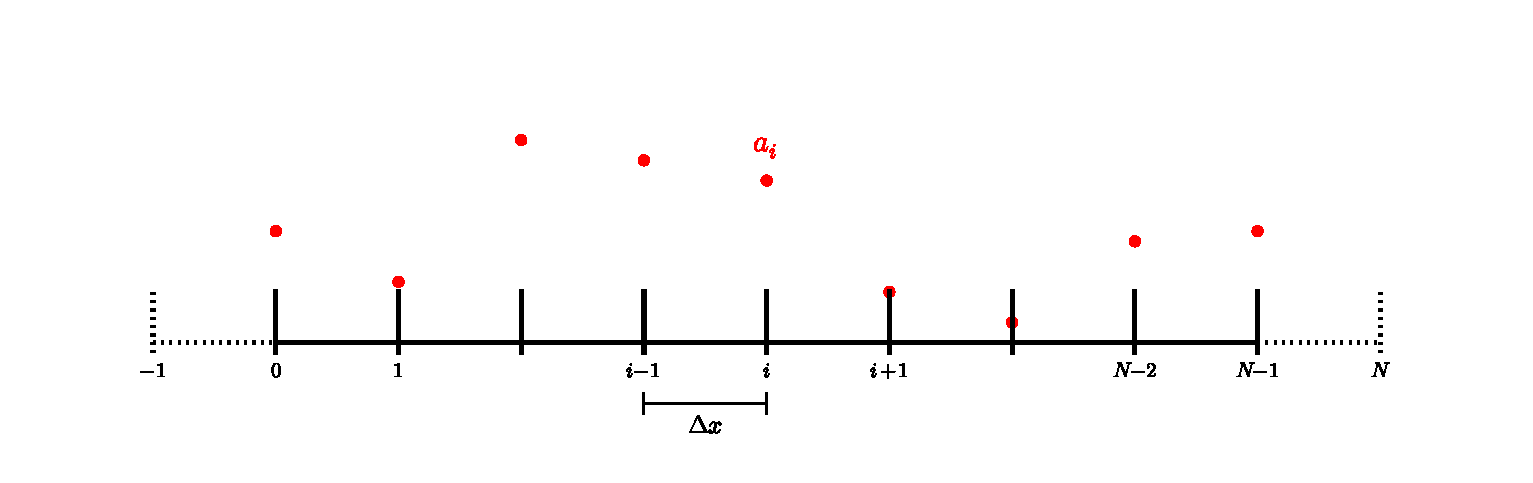
\includegraphics[width=7.0in]{fd_ghost}
\caption{\label{fig:fdgrid} A simple finite-difference grid.  The solution
  is stored at each of the labeled points.  The dotted lines show the
  ghost points used to extend our grid past the physical boundaries to 
  accommodate boundary conditions.  Note that if we are periodic, then
  points $0$ and $N-1$ are at the same physical point in space, so we
  would only need to update one of them.}
\end{figure}

The last piece of information needed to update the solution is the
timestep, $\Delta t$.  It can be shown that for the solution to be
{\em stable}, the timestep must be less than the time it takes information
to propagate across a single zone.  That is:
\begin{equation}
\Delta t \le \frac{\Delta x}{u} \enskip .
\end{equation}
This is called the {\em Courant-Friedrichs-Lewy} or {\em CFL}
condition.  A dimensionless quantity called the {\em CFL number} is 
defined as 
\begin{equation}
C = \frac{\Delta t u }{\Delta x} 
\end{equation}
Stability requires $C \le 1$.
%
We traditionally write the timestep as
\begin{equation}
\label{eq:timestep}
\Delta t = C \frac{\Delta x}{u}
\end{equation}
and specify $C$ as part of the problem (a typical value may be $C = 0.7$).

\begin{quote}
{\em Exercise 2: Show analytically that when you use $C=1$ in the
  first-order differenced advection equation (Eq.~\ref{eq:fo}) that
  you advect the profile exactly, without any numerical error.}
\end{quote}

Keep in mind that, in general, we will be solving a non-linear
system of equations, so it is not possible to run with $C=1$, 
since $u$ (and therefore $C$) will change from zone to zone.
Instead, one looks at the most restrictive timestep over all the
zones and uses that for the entire system.


\begin{quote}
{\em Exercise 3: Write a code to solve the 1-d linear advection equation
  using the discretization of Eq.~\ref{eq:fo} on the domain $[0,1]$ with
  $u=1$ and periodic boundary conditions.  For initial conditions,
  try both a Gaussian profile and a top-hat:}
  \begin{equation}
  a = \left \{
      \begin{array}{lllll}0 & \mathit{~if~~} &         &x& < 1/3 \\
                          1 & \mathit{~if~~} & 1/3 \le &x& < 2/3 \\
                          0 & \mathit{~if~~} & 2/3 \le &x&
      \end{array}
      \right .
  \end{equation}

  {\em Note: For a general treatment of boundary conditions, you would
    initialize the ghost points to their corresponding periodic data
    and apply the difference equations to zones $0, \ldots, N-1$.
    However, for periodic BCs on this grid, points $0$ and $N-1$ are
    identical, so you could do the update in this special case on
    points $1, \ldots, N-1$ without the need for ghost points and then
    set $a_0 = a_{N-1}$ after the update.}

  \noindent {\em Run you program for one or more periods (one period
    is $T=1/u$) with several different CFL numbers and notice that
    there is substantial numerical dissipation.}
\end{quote}


\begin{quote}
{\em Exercise 4: You may think that using a centered-difference for
  the spatial derivative, $u_x \sim (u_{i+1} - u_{i-1})/(2 \Delta x)$
  would be more accurate.  This method is called FTCS (forward-time,
  centered-space).  Try this.  You will find that the solution is
  unconditionally unstable.  }
\end{quote}

The classic method for understanding stability is to consider the growth 
of a single Fourier mode in our discetization.  That is, substitute in
$a_i^n = A^n e^{ji\theta}$, where $j = \sqrt{-1}$, and $\theta$ represents a
phase.  A method is stable if $|A^{n+1}/A^n| \le 1$.  Performing this
with FTCS shows that no value of $C$ can make the method stable.
Doing the same analysis for Eq.~\ref{eq:fo} would show that the upwind
method is stable for $0\le C \le 1$. 
(Note that this stability analysis only works for linear equations, where
the difference Fourier modes are decoupled, nevertheless, we use its
ideas for nonlinear advection problems as well).

\begin{quote}
{\em Exercise 5: To get an alternate feel for stability, we can ask
  what the terms left out by truncation look like.  That is, we can
  begin with the discretized equation:
\begin{equation}
  a_i^{n+1} - a_i^n = -\frac{u \Delta t}{\Delta x} ( a_i^n - a_{i-1}^n )
\end{equation}
and replace $a_i^{n+1}$ with a Taylor expansion in time, and replace
$a_{i-1}^n$ with a Taylor expansion in space, keeping terms to
$O(\Delta t^3)$ and $O(\Delta x^3)$.  Replacing $\partial a/\partial t$
with $-u \partial a/ \partial x$ in the higher-order terms, show 
that our difference equation more closely corresponds to 
\begin{eqnarray}
a_t + u a_x &=& \frac{u \Delta x}{2} \left ( 1 - \frac{\Delta t u}{\Delta x} \right ) \frac{\partial^2 a}{\partial x^2} \\
            &=& \frac{u \Delta x}{2} (1 - C) \frac{\partial^2 a}{\partial x^2}
\end{eqnarray}

Notice that the righthand side looks like a diffusion term, however,
if $C > 1$, then the coefficient of the diffusion is negative---this is
unphysical.  This means that the diffusion would act to take smooth
features and make them more strongly peaked---the opposite of physical
diffusion.

}
\end{quote}

An alternate approach to time-discretization is to do an implicit
discretization.  Here our upwind method would appear as:
\begin{equation}
\frac{a^{n+1}_i - a^n_i}{\Delta t} = -u \frac{a^{n+1}_i - a^{n+1}_{i-1}}{\Delta x}
\end{equation}
We can write this as a linear system with coupled equations:
\begin{equation}
-C a^{n+1}_{i-1} + (1 + C) a^{n+1}_i = a_i^n
\end{equation}
This requires a matrix solve---this makes implicit methods generally more
expensive than explicit methods.  However, stability analysis would show
that this implicit discretization is stable for any choice of $C$. (But
one must not confuse stability with accuracy---the most accurate solutions
with this method will still have a small $C$).

%%%%%%%%%%%%%%%%%%%%%%%%%%%%%%%%%%%%%%%%%%%%%%%%%%%%%%%%%%%%%%%%%%%%%%%%%%%%%%
\section{Second-order advection in one-dimension and the finite-volume method}

We will typically use a {\em finite-volume} discretization of the
advection equation.  First we rewrite the advection equation in {\em
  conservation form}:
\begin{equation}
a_t + \left[f(a)\right]_x = 0
\label{eq:advect-cons}
\end{equation}
where $f(a) = ua$ is the flux of the quantity $a$.  In conservation form,
the time derivative of a quantity is related to the divergence of 
its flux.

\begin{figure}
\centering
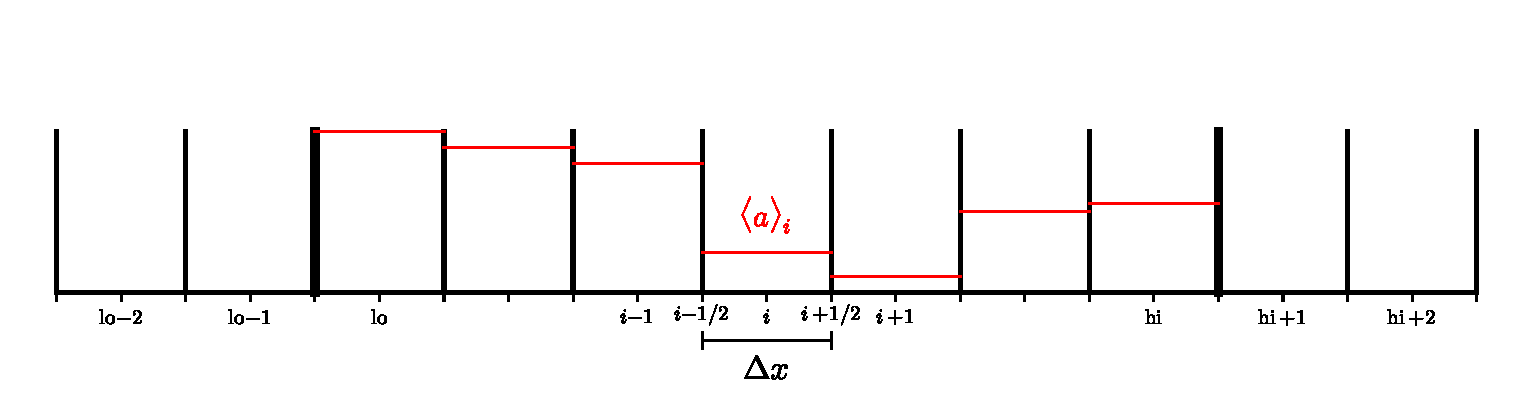
\includegraphics[width=6.4in]{fv_ghost}
\caption{\label{fig:fvghost} A finite-volume grid running from
  $\mathrm{lo}, \ldots, \mathrm{hi}$, with two ghost cells at each
  end.}
\end{figure}

Recall that in the finite-volume discretization, $\langle a\rangle_i$
represents the average of $a(x,t)$ over the interval $x_{i-1/2}$ to
$x_{i+1/2}$, where the half-integer indexes denote the zone edges
(i.e.\ $x_{i-1/2} = x_i - \Delta x/2$).  Figure~\ref{fig:fvghost}
shows an example of such a grid with 2 ghost cells at each end.  (For
simplicitly of notation, we drop the $\langle \rangle$ going forward).
To discretize Eq.~\ref{eq:advect-cons}, we integrate it over a zone,
from ${x_{i-1/2}}$ to ${x_{i+1/2}}$, normalizing by the zone width,
$\Delta x$:
\begin{eqnarray}
\frac{1}{\Delta x} \int_{x_{i-1/2}}^{x_{i+1/2}} a_t \, dx &=& 
   - \frac{1}{\Delta x} \int_{x_{i-1/2}}^{x_{i+1/2}} \frac{\partial}{\partial x} f(a) \, dx \\
\frac{\partial}{\partial t} a_i &=& 
   - \frac{1}{\Delta x} \left \{ \left [f(a) \right ]_{i+1/2} - \left [f(a) \right ]_{i-1/2} \right \}
\end{eqnarray}
This is an evolution equation for the zone-average of $a$, and shows
that it updates in time based on the fluxes through the boundary of
the zone.  We discretize in time by evaluating the righthand side at
the midpoint in time---this gives a centered difference in time, which
is second-order accurate:
\begin{equation}
\frac{a_i^{n+1} - a_i^n}{\Delta t} = -\frac{\left [f(a) \right ]_{i+1/2}^{n+1/2} - \left [f(a) \right ]_{i-1/2}^{n+1/2}}{\Delta x}
\label{eq:consupdate1d}
\end{equation}
To evaluate the fluxes at the half-time, we need the state at the
half-time, that is, we do :
\begin{equation}
\left [f(a) \right ]_{i+1/2}^{n+1/2} = f(a_{i+1/2}^{n+1/2}) \enskip .
\end{equation}
We construct a second-order accurate approximation to
$a_{i+1/2}^{n+1/2}$ by Taylor expanding the data in the cell to the
interface.  Note that for each interface, there are two possible
interface states we can construct---one using the data to the left of
the interface (which we will denote with a ``L'' subscript) and the
other using the data to the right of the interface (denoted with an
``R'' subscript)---see Figure~\ref{fig:riemann}.  These states are:
\begin{eqnarray}
a_{i+1/2,L}^{n+1/2} &=& a_i^n + \frac{\Delta x}{2} \left .\frac{\partial a}{\partial x} \right |_i + \frac{\Delta t}{2} \left .\frac{\partial a}{\partial t} \right |_i + \mathcal{O}(\Delta x^2) + \mathcal{O}(\Delta t^2) \nonumber \\
    &=& a_i^n + \frac{\Delta x}{2} \left .\frac{\partial a}{\partial x} \right |_i +  \frac{\Delta t}{2} \left ( - u \left .\frac{\partial a}{\partial x} \right |_i \right ) + \ldots \nonumber \\
    &=& a_i^n + \frac{\Delta x}{2} \left ( 1 - \frac{\Delta t}{\Delta x} u \right ) \left .\frac{\partial a}{\partial x} \right |_i +  \ldots \label{eq:statel}\\
%%
a_{i+1/2,R}^{n+1/2} &=& a_{i+1}^n - \frac{\Delta x}{2} \left .\frac{\partial a}{\partial x} \right |_{i+1} + \frac{\Delta t}{2} \left .\frac{\partial a}{\partial t} \right |_{i+1} + \mathcal{O}(\Delta x^2) + \mathcal{O}(\Delta t^2) \nonumber \\
    &=& a_{i+1}^n - \frac{\Delta x}{2} \left .\frac{\partial a}{\partial x} \right |_{i+1} +  \frac{\Delta t}{2} \left ( - u \left .\frac{\partial a}{\partial x} \right |_{i+1} \right ) + \ldots \nonumber \\
    &=& a_{i+1}^n - \frac{\Delta x}{2} \left ( 1 + \frac{\Delta t}{\Delta x} u \right ) \left .\frac{\partial a}{\partial x} \right |_{i+1} +  \ldots \label{eq:stater}
\end{eqnarray}
\begin{figure}[t]
\centering
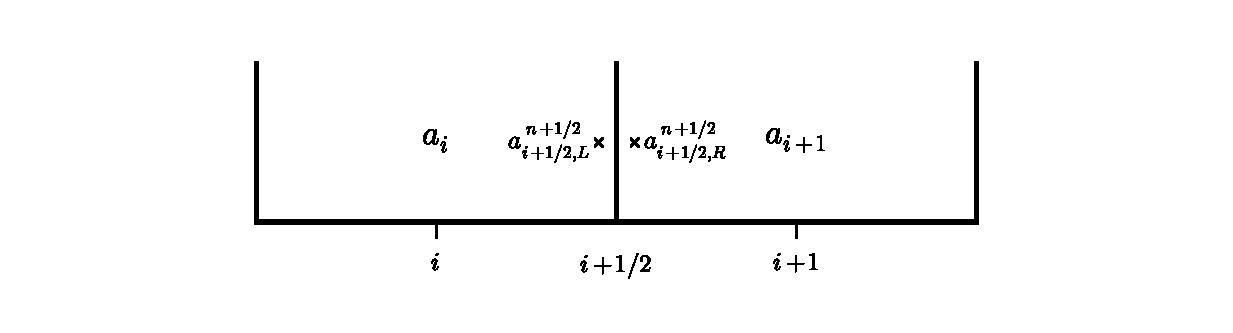
\includegraphics[width=5.0in]{riemann}
\caption{\label{fig:riemann} The left and right interface state at the
  $i+1/2$ interface.  Here, the left state, $a_{i+1/2,L}^{n+1/2}$, was
  predicted to the interface from the zone to the left of the
  interface, using $a_i$, and the right state, $a_{i+1/2,R}^{n+1/2}$,
  was predicted to the interface from the zone to the right, using
  $a_{i+1}$.}
\end{figure}

A suitable estimate is needed for the slope of $a$ that appears in these 
expressions (as $\partial a/\partial x$).  We can approximate this simply
as 
\begin{equation}
\left . \frac{\partial a}{\partial x}\right |_i = \frac{a_{i+1} - a_{i-1}}{2 \Delta x} \label{eq:slopecentered}
\end{equation}

We can think of this method as reconstructing the function form of the
data from the cell-average data in each cell using  a piecewise linear
polynomial. 

We now have two states, $a_{i+1/2,L}^{n+1/2}$ and
$a_{i+1/2,R}^{n+1/2}$ separated by an interface---this is called the
{\em Riemann problem}.
%
The solution to this will depend on the equation being solved, and
results in a single state at the interface:
\begin{equation}
a_{i+1/2}^{n+1/2} = \mathcal{R}(a_{i+1/2,L}^{n+1/2},a_{i+1/2,R}^{n+1/2})
\end{equation}
In our case, the advection equation simply propagates the state to the
right (for $u > 0$), so the solution to the Riemann problem is to take
the left state (this is another example of upwinding).  That is we do:
\begin{equation}
\mathcal{R}(a_{i+1/2,L}^{n+1/2},a_{i+1/2,R}^{n+1/2}) = \left \{ \begin{array}{ccc} a_{i+1/2,L}^{n+1/2} & u > 0 \\[2mm] a_{i+1/2,R}^{n+1/2} & u < 0 \end{array} \right .
\label{eq:riemannsolve}
\end{equation}
To complete the update, we use this interface state to evaluate the flux
and update the advected quantity via Eq.~\ref{eq:consupdate1d}.

Boundary conditions are implemented by filling the ghost cells outside
each end of the domain based on data in the interior.  Note that at
the very left edge of the domain, the state
$a^{n+1/2}_{\mathrm{lo}-1/2}$ requires the construction of states on
the left and right.  The left state at that interface,
$a^{n+1/2}_{\mathrm{lo}-1/2,L}$ depends on the slope reconstructed in
the $\mathrm{lo}-1$ ghost cell, $\partial a/\partial x
|_{\mathrm{lo}-1}$.  This in turn is constructed using a limited
center-difference that will consider the value in the cell to the
left, $\mathrm{lo-2}$.  Therefore, we need two ghost cells at each end
of the domain for this method.  Higher-order limiters may require even
more ghost cells.

\begin{quote}
{\em Exercise 6: Write a second-order solver for the linear advection
  equation.  To mimic a real hydrodynamics code, your code should have
  routines for finding initializing the state, filling boundary conditions,
  computing the timestep,
  computing the interface states, solving the Riemann problem, and
  doing the update.  The problem flow should look like:
  \begin{itemize}
    \item set initial conditions
    \item main evolution loop---loop until final time reached
    \begin{itemize}
      \item fill boundary conditions
      \item get timestep (Eq.~\ref{eq:timestep})
      \item compute interface states (Eqs.~\ref{eq:statel} and \ref{eq:stater})
      \item solve Riemann problem at all interfaces (Eq.~\ref{eq:riemannsolve})
      \item do conservative update (Eq.~\ref{eq:consupdate1d})
    \end{itemize}
  \end{itemize}
Use both the top-hat and Gaussian initial conditions and periodic boundary
conditions and compare to the first-order method.
}
\end{quote}

\subsection{Limiting}

The second-order method likely showed some oscillations in the
solution, especially for the top-hat initial conditions.  {\em
  Godunov's theorem} says that any monotonic linear method for
advection is first-order accurate (see, e.g,~\cite{laney}).  In this
context, monotonic means that no new minima or maxima are introduced.
The converse is true too, which suggests that in order to have a
second-order accurate method for this linear equation, the algorithm
itself must be nonlinear.

\begin{quote}
{\em Exercise 7:   To remove the oscillations in
practice, we limit the slopes to ensure that no new minima or maxima are
introduced during the advection process.  There are many choices for
limited slopes.  A popular one is the {\em minmod} limiter.  Here, we
construct the slopes in the interface states as:
\begin{equation}
\left . \frac{\partial a}{\partial x} \right |_i = \mathtt{minmod} \left (
  \frac{a_i - a_{i-1}}{\Delta x}, \frac{a_{i+1} - a_i}{\Delta x} \right )
\end{equation}
instead of Eq.~\ref{eq:slopecentered}.
with 
\begin{equation}
\mathtt{minmod}(a,b) = \left \{ 
    \begin{array}{ll}
    a & \mathit{if~} |a| < |b| \mathrm{~and~} a\cdot b > 0 \\
    b & \mathit{if~} |b| < |a| \mathrm{~and~} a\cdot b > 0 \\
    0 & \mathit{otherwise}
    \end{array}
  \right .
\end{equation}
Use this slope in your second-order advection code and notice that the
oscillations go away }
\end{quote}

Figure~\ref{fig:limitingex} shows the evolution
of an initial discontinuity with and without limiting.  See the text
by LeVeque~\cite{leveque:2002} for alternate choices of
limiters. Note: most limiters will have some sort of test on the product
of a left-sided and right-sided difference ($a\cdot
b$ above)---this is $< 0$ at an extremum, which is precisely where we want to
limit. 

\begin{figure}[p!]
\centering
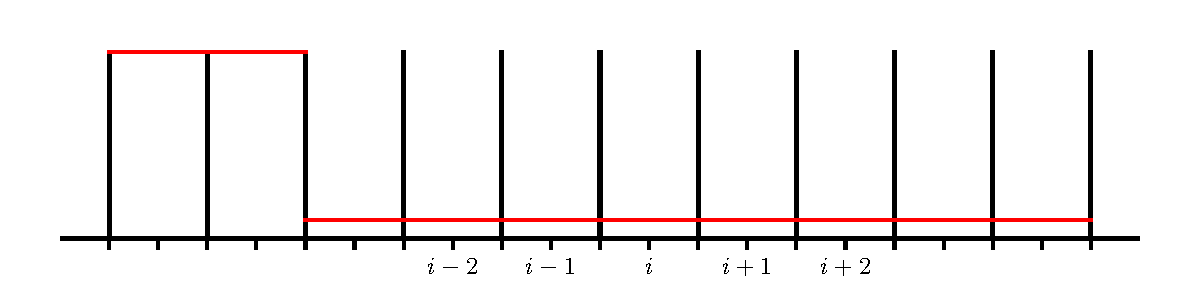
\includegraphics[width=3.25in]{rea-nolimit-start_001}\hspace{1em}
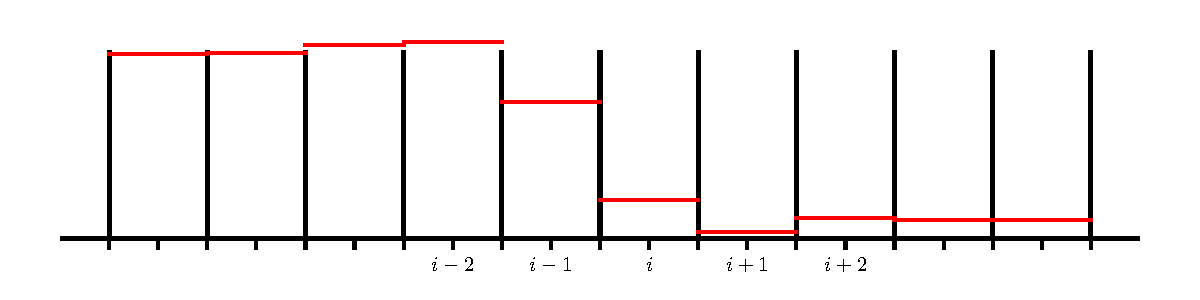
\includegraphics[width=3.25in]{rea-nolimit-start_005} \\
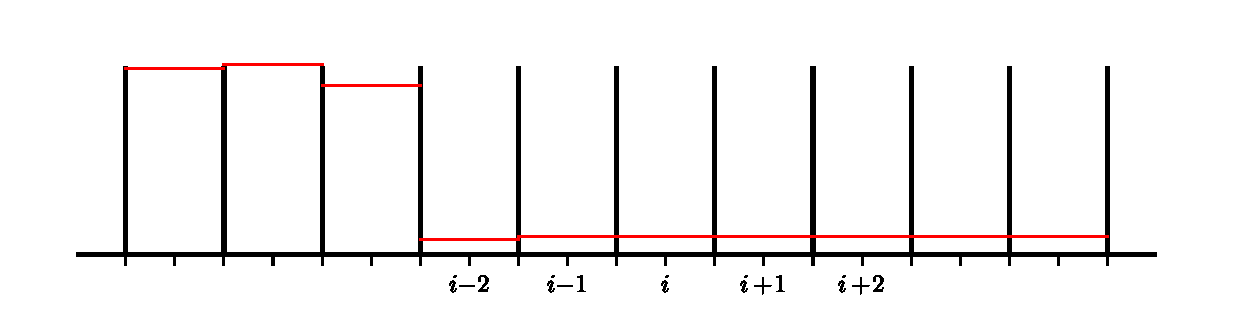
\includegraphics[width=3.25in]{rea-nolimit-start_002}\hspace{1em}
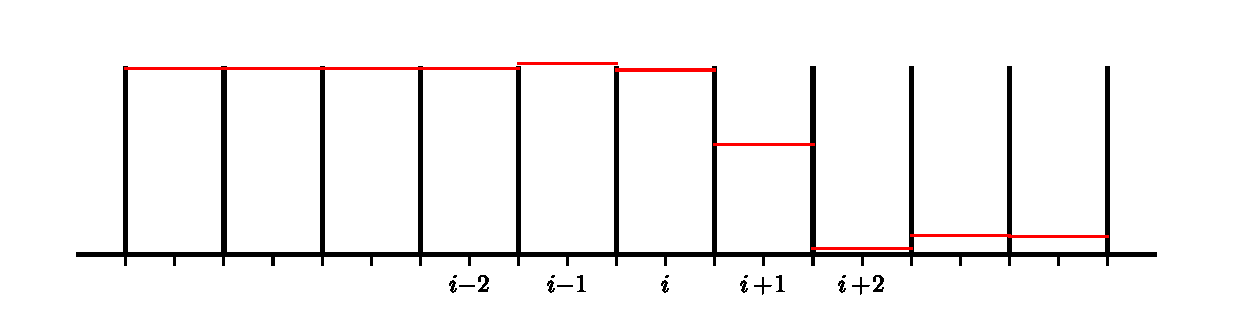
\includegraphics[width=3.25in]{rea-nolimit-start_006} \\
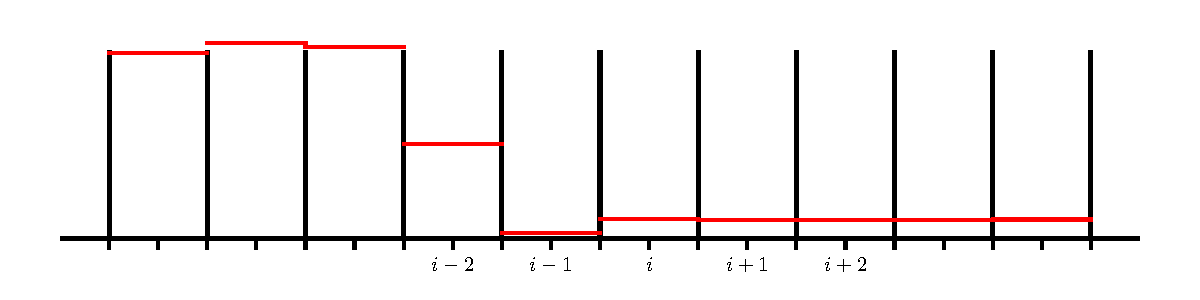
\includegraphics[width=3.25in]{rea-nolimit-start_003}\hspace{1em}
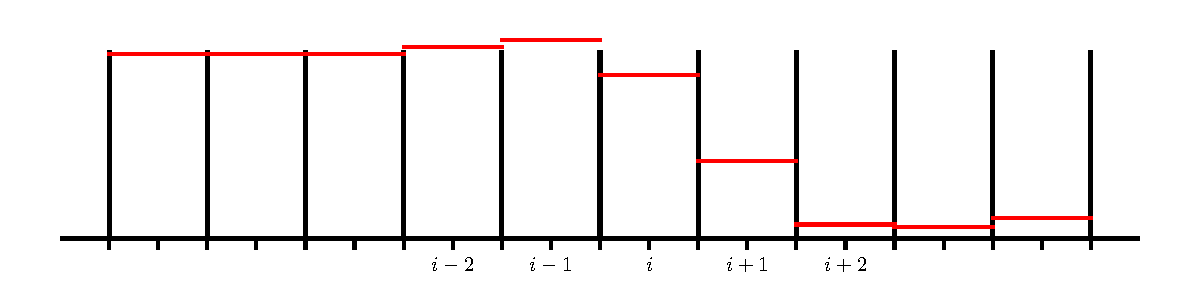
\includegraphics[width=3.25in]{rea-nolimit-start_007} \\
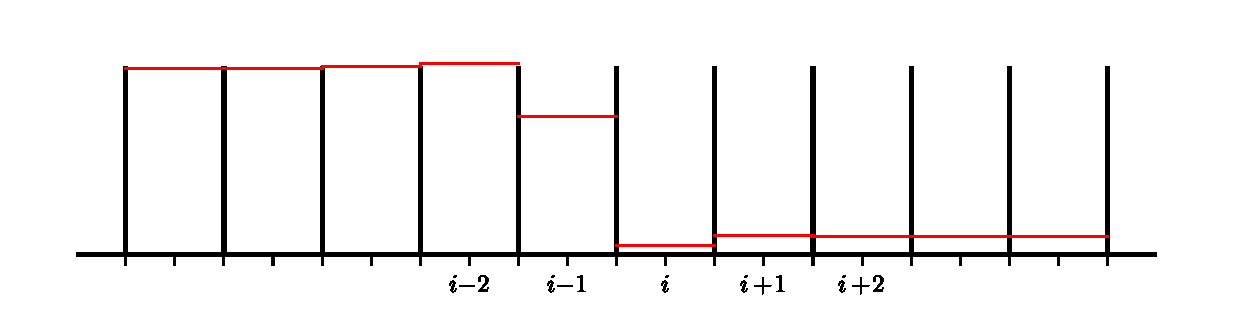
\includegraphics[width=3.25in]{rea-nolimit-start_004}\hspace{1em}
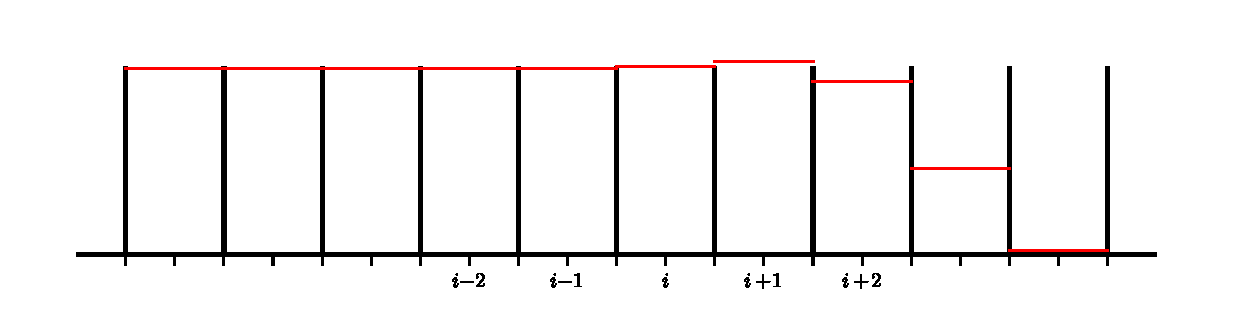
\includegraphics[width=3.25in]{rea-nolimit-start_008} \\
\vskip 0.5in
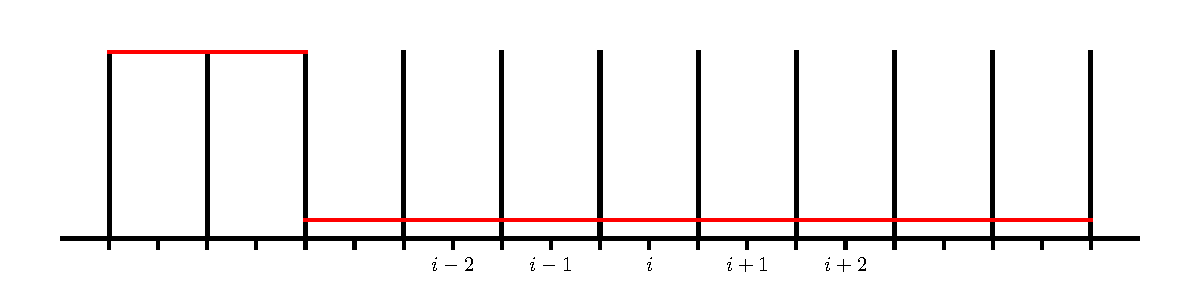
\includegraphics[width=3.25in]{rea-start_001}\hspace{1em}
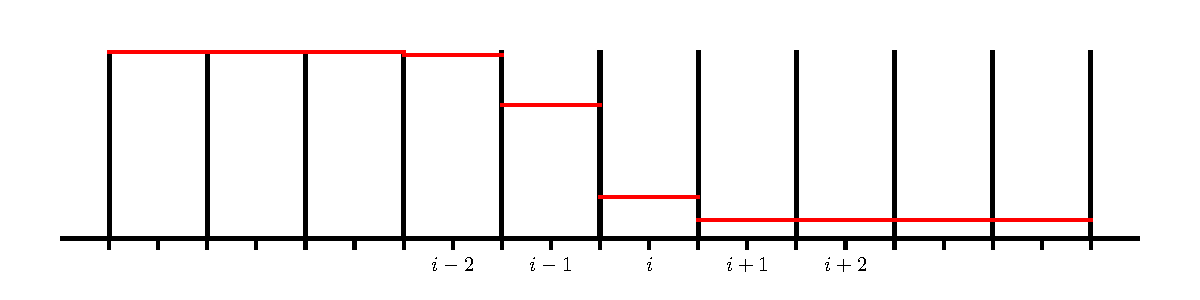
\includegraphics[width=3.25in]{rea-start_005} \\
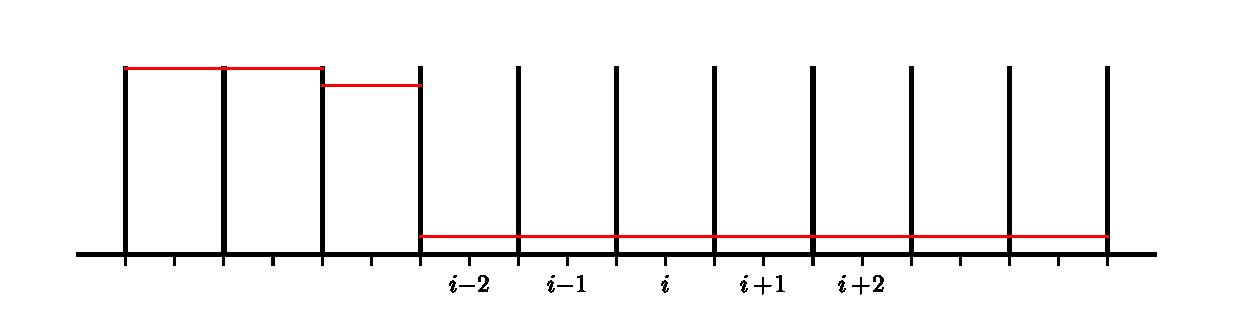
\includegraphics[width=3.25in]{rea-start_002}\hspace{1em}
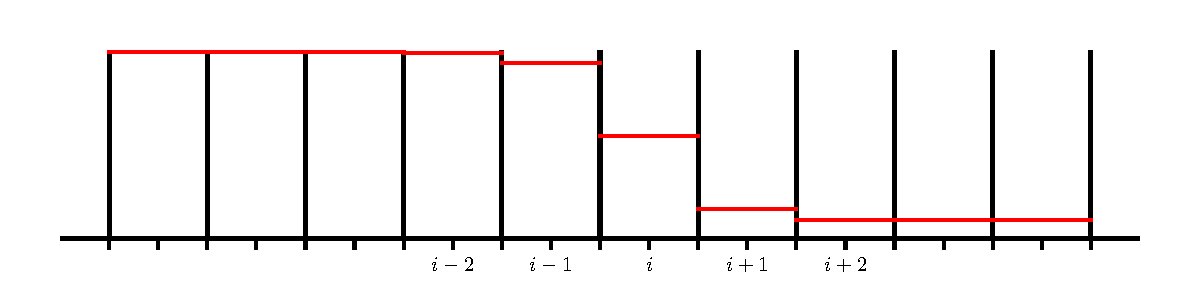
\includegraphics[width=3.25in]{rea-start_006} \\
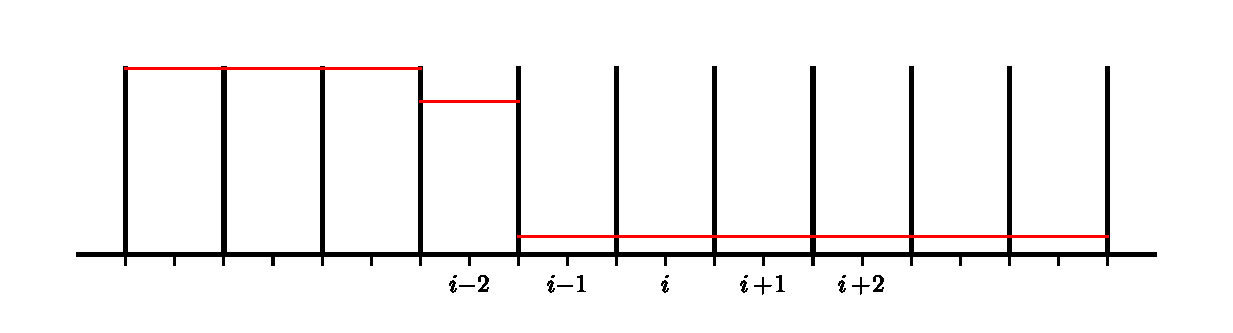
\includegraphics[width=3.25in]{rea-start_003}\hspace{1em}
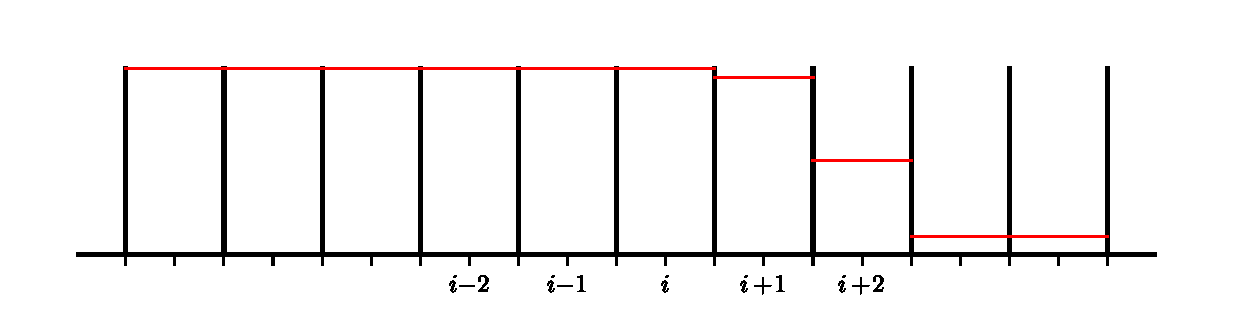
\includegraphics[width=3.25in]{rea-start_007} \\
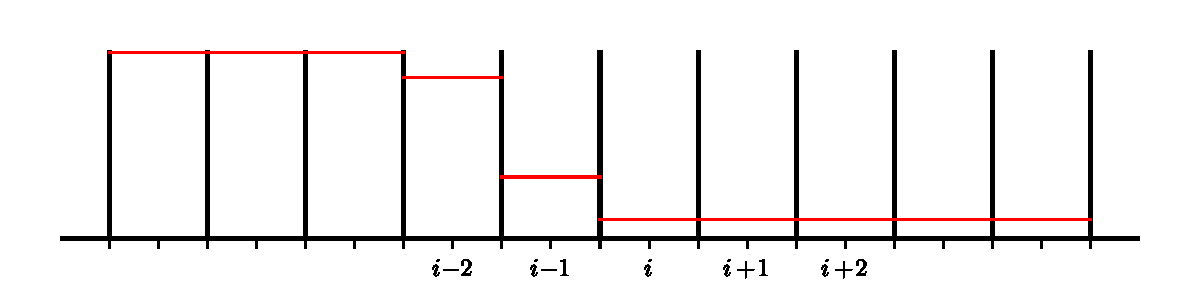
\includegraphics[width=3.25in]{rea-start_004}\hspace{1em}
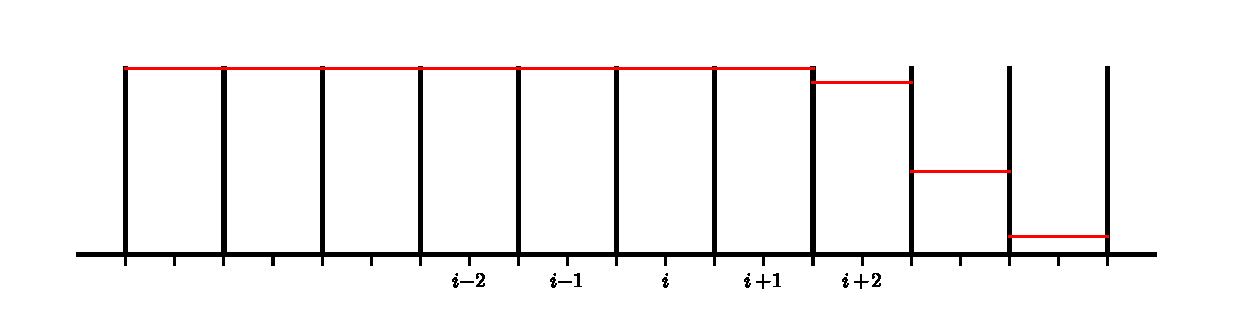
\includegraphics[width=3.25in]{rea-start_008} \\
\caption{\label{fig:limitingex}Initially discontinuous data evolved for several steps with
  no limiting (top sequence) and limiting (bottom sequence).  Note
  that without limiting, there are overshoots and undershoots
  surrounding the discontinuity, and that the discontinuity remains
  sharper with limiting.}
\clearpage
\end{figure}

A slightly more complex limiter is the MC limiter (monotonized central
difference).  First we define an extrema test,
\begin{equation}
\xi = (a_{i+1} - a_i) \cdot (a_i - a_{i-1})
\end{equation}
Then the limited difference is
\begin{equation}
\left . \frac{\partial a}{\partial x} \right |_i = 
 \left \{
\begin{array}{ll}
\min \left [ \frac{| a_{i+1} - a_{i-1} |}{2 \Delta x},
              2 \frac{| a_{i+1} - a_i |}{\Delta x},
              2 \frac{| a_{i} - a_{i-1} |}{\Delta x}
      \right ]  \mathrm{sign}(a_{i+1} - a_{i-1}) &  \xi > 0 \\
0 & \mathit{otherwise}
\end{array}
\right .
\end{equation}
%
This is second-order accurate for smooth flows.  

The main goal of a limiter is to reduce the slope near extrema.
Figure~\ref{fig:limit} shows a finite-volume grid with the original
data, cell-centered slopes, and MC limited slopes.  Note that near the
strong gradients is where the limiting kicks in.  The different limiters
are all constructed by enforcing a conditions requiring the method to be
{\em total variation diminishing}, or TVD.  More details on TVD limiters
can be found in \cite{toro:1997,leveque:2002}.

\begin{figure}
\centering
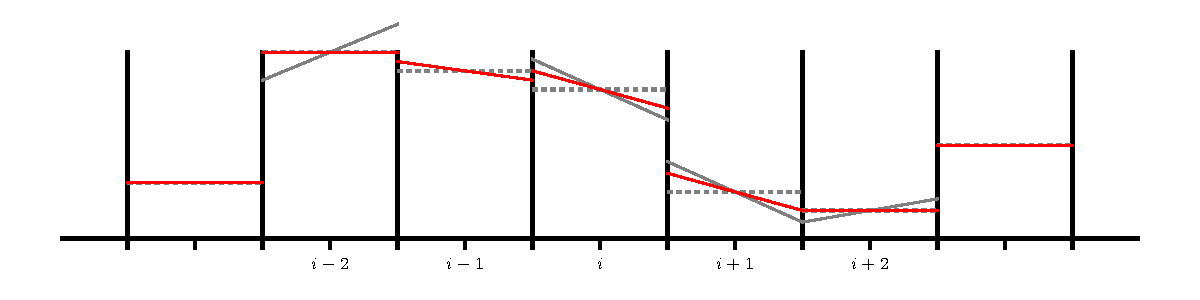
\includegraphics[width=6.0in]{generalgrid}
\caption{\label{fig:limit} A finite-volume grid showing the cell
  averages (gray horizontal lines), unlimited center-difference slopes
  (blue) and MC limited slopes (red).  Note that in zones $i$ and
  $i+1$, the slopes are limited slightly, so as not to overshoot or
  undershoot the neighboring cell value.  Cell $i-1$ is not limited at
  all, whereas cells $i-2$, and $i+2$ are fully limited---the slope is
  set to 0---these are extrema.}
\end{figure}

A popular extension of the MC limiter is the $4^\mathrm{th}$-order MC
limiter, which is more accurate in smooth flows (this is shown in
\cite{colella:1985}, Eqs. 2.5 and 2.6; and \cite{colella:1990},
Eq. 191).

\begin{quote}
{\em Exercise 8: Show analytically that if you fully limit the slopes
  (i.e.\ set $\partial a/\partial x |_i = 0$, that the second-order
  method reduces to precisely our first-order finite-difference discretization,
  Eq.~\ref{eq:fo}.  }
\end{quote}


%%%%%%%%%%%%%%%%%%%%%%%%%%%%%%%%%%%%%%%%%%%%%%%%%%%%%%%%%%%%%%%%%%%%%%%%%%%%%%
\subsection{Reconstruct-evolve-average}

Another way to think about these methods is as a reconstruction,
evolve, and average (R-E-A) process (see Figure~\ref{fig:rea}).  

We can write the conservative update as:
\begin{eqnarray}
a_i^{n+1} &=& a_i^n + \frac{\Delta t}{\Delta x} 
    (u a^{n+1/2}_{i-1/2} - u a^{n+1/2}_{i+1/2} ) \\
          &=& a_i^n + C (a^{n+1/2}_{i-1/2} - a^{n+1/2}_{i+1/2} ) 
\end{eqnarray}
If we take $u > 0$, then the Riemann problem will always choose the
left state, so we can write this as:
\begin{equation}
a_i^{n+1} = a_i^n + 
     C \left [\left (a_{i-1}^n + \frac{1}{2} (1-C) \Delta a_{i-1} \right ) -
              \left (a_{i}^n + \frac{1}{2} (1-C) \Delta a_{i} \right ) 
       \right ] \label{eq:rea_orig}
\end{equation}

If we instead look at this via the R-E-A procedure, we write the reconstructed
$a$ in each zone in the form of a piecewise linear polynomial
\begin{equation}
a_i(x) = a_i + \frac{\Delta a}{\Delta x} (x - x_i)
\end{equation}
Consider zone $i$.  
If we are advecting with a CFL number $C$, then that means that the fraction
$C$ of the zone immediately to the left of the $i-1/2$ interface will advect
into zone $i$ over the timestep.  And only the fraction $1-C$ in zone $i$
immediately to the right of the interface will stay in that zone.  This 
is indicated by the shaded regions in Figure~\ref{fig:rea}. 

The average of the quantity $a$ from zone $i-1$ that will advect into
zone $i$ is 
\begin{eqnarray}
\mathcal{I}_< &=& \frac{1}{C \Delta x} 
   \int_{x_{i-1/2} - C\Delta x}^{x_{i-1/2}} a_{i-1}(x) dx \\
%
 &=& \frac{1}{C \Delta x} 
   \int_{x_{i-1/2} - C\Delta x}^{x_{i-1/2}}
        \left [ a_{i-1} + \frac{\Delta a_{i-1}}{\Delta x} (x - x_{i-1} ) \right ] dx  \\
 &=& a_{i-1} + \frac{1}{2} \Delta a_{i-1} (1-C)
\end{eqnarray}

And the average of the quantity $a$ in zone $i$ that will remain in zone $i$
is
\begin{eqnarray}
\mathcal{I}_> &=& \frac{1}{(1-C) \Delta x} 
   \int_{x_{i-1/2}}^{x_{i-1/2} + (1-C) \Delta x} a_{i}(x) dx \\
%
 &=& \frac{1}{(1-C) \Delta x} 
   \int_{x_{i-1/2}}^{x_{i-1/2} + (1-C)\Delta x} 
        \left [ a_{i} + \frac{\Delta a_{i}}{\Delta x} (x - x_{i} ) \right ] dx  \\
 &=& a_{i} - \frac{1}{2} \Delta a_{i} C
\end{eqnarray}

The final part of the R-E-A procedure is to average the over the 
advected profiles in the new cell.  The weighted average of the
average brought in from the left of the interface and that that remains
in the cell is
\begin{equation}
a_i^{n+1} = C \mathcal{I}_< + (1 - C) \mathcal{I}_> 
\end{equation}          
This is identical to Eq.~\ref{eq:rea_orig}.  This demonstrates that the
R-E-A procedure is equivalent to our reconstruction, prediction of the
interface states, solving the Riemann problem, and doing the 
conservative flux update.

\begin{figure}
\centering
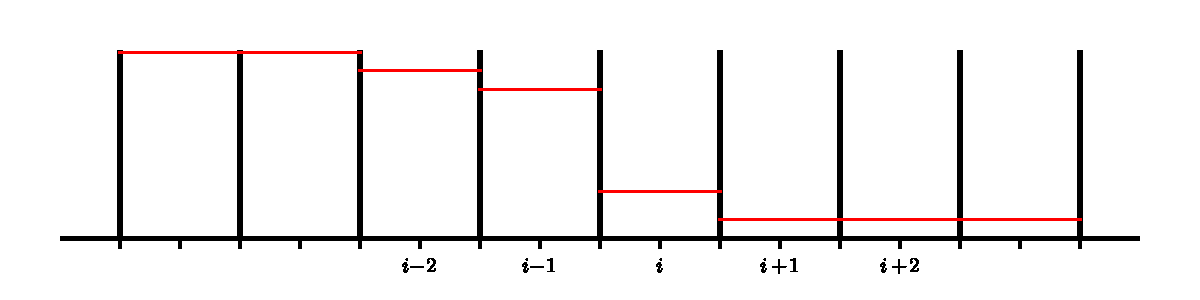
\includegraphics[width=6.0in]{rea-start} \\
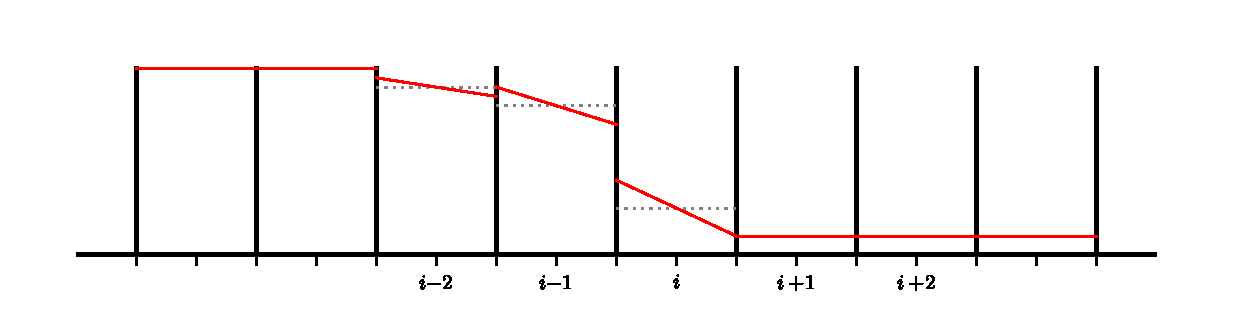
\includegraphics[width=6.0in]{rea-reconstruction.eps} \\
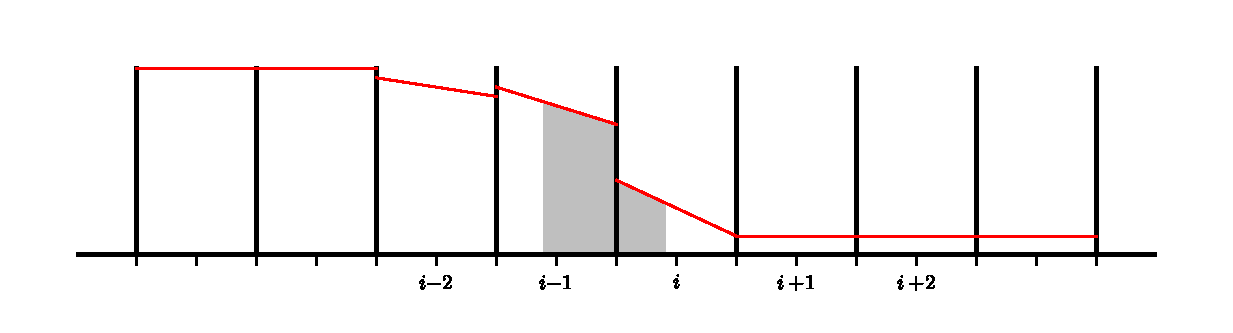
\includegraphics[width=6.0in]{rea-trace.eps} \\
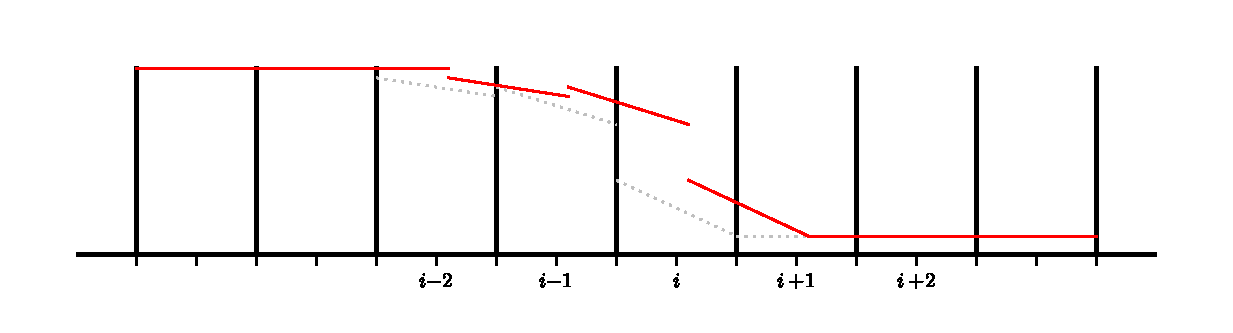
\includegraphics[width=6.0in]{rea-evolve.eps} \\
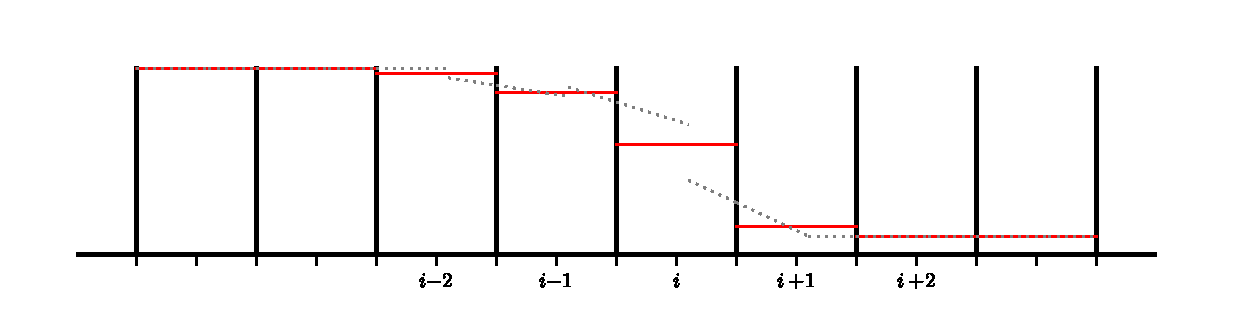
\includegraphics[width=6.0in]{rea-final.eps}
\caption{\label{fig:rea} Reconstruct-Evolve-Average.  The top panel
  shows the origina cell-average data.  The second panel shows the
  (limited) piecewise linear reconstruction of the data.  Assuming a
  CFL number of 0.6 and advection to the right, the shaded regions
  in the third panel show the data that will wind up in cell $i$
  after advecting for a single step.  The fourth panel shows the
  piecewise-linear data advected to the right by 0.6 of a cell-width
  (corresponding to a CFL of 0.6).  The final panel shows the new
  averages of the data, constructed by averaging the advected 
  piecewise linear data in each cell.}
\end{figure}




%%%%%%%%%%%%%%%%%%%%%%%%%%%%%%%%%%%%%%%%%%%%%%%%%%%%%%%%%%%%%%%%%%%%%%%%%%%%%%
\section{Errors and convergence rate}

For the advection problem, the analytic solution is to simply propagate
the initial profile to the right.  This means that with periodic boundary
condition, after advecting for one period, our numerical solution should
be identical to the initial conditions.  Any differences are our
numerical error.  We can quantify the error by taking the norm of error as:
This is the {\em L2-norm} of the relative error.  Sometimes we instead look
at the norm of the absolute error:
\begin{equation}
\epsilon^\mathrm{abs} = \| a^\mathrm{final} - a^\mathrm{init} \|_2 \equiv
   \left [ \frac{1}{N} \sum_{i=1}^N 
   ( a_i^\mathrm{final} - a_i^\mathrm{init} )^2
  \right ]^{1/2}
\end{equation}
It is sometimes useful to compare to the norm of the original solution
to get a measure of the relative error:
\begin{equation}
\epsilon^\mathrm{rel} \equiv \frac{\| a^\mathrm{final} - a^\mathrm{init} \|_2}
   {\| a^\mathrm{init} \|_2}
\end{equation}
Note that it is important in these definitions to normalize by the number
of zones, $N$, otherwise our error will be resolution-dependent.
%
\begin{quote}
{\em Exercise 9: Run the first-order solver for several different $\Delta x$s,
each a factor of 2 smaller than the previous.  Compute $\epsilon$ for
each resolution and observe that it converges in a first-order fashion
(i.e.\ $\epsilon$ decreases by 2 when we decrease $\Delta x$ by a factor of 2).

Do the same with the second-order solver and observe that it converges
as second-order.
}
\end{quote}

\section{Multi-dimensional advection}

The two-dimensional linear advection equation is:
\begin{equation}
a_t + u a_x + v a_y = 0
\label{eq:advect2d}
\end{equation}
where $u$ is the velocity in the $x$-direction and $v$ is the velocity in
the $y$-direction.  We denote the average of $a(x,y,t)$ in a zone $i,j$ as
$a_{i,j}$.  Here, $i$ is the index in the $x$-direction and $j$ is the
index in the $y$-direction.  A 2-d grid is shown in Figure~\ref{fig:2dgrid}.
Just as in the one-dimensional case, we will extend the domain with a
perimeter of ghost cells to set the boundary conditions.

\begin{figure}[h]
\centering
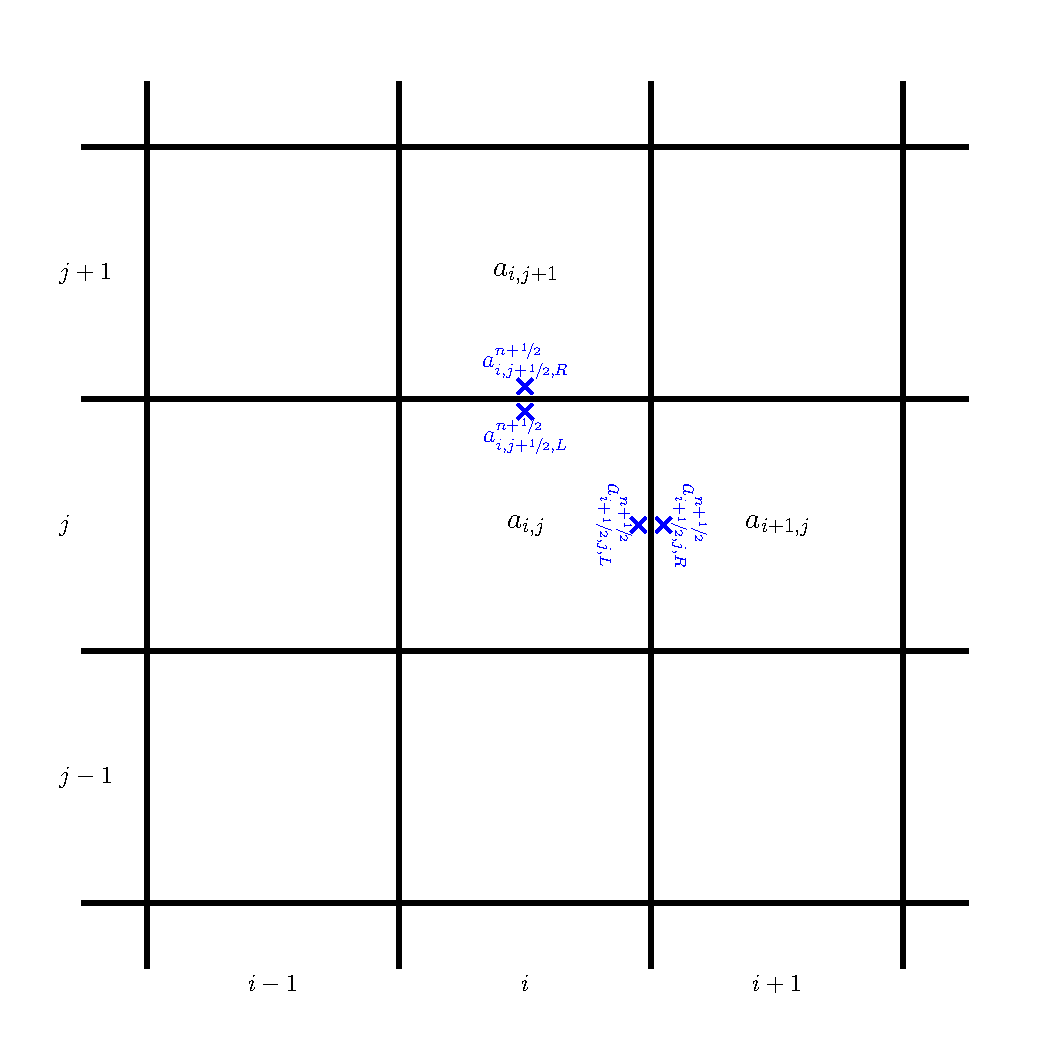
\includegraphics[width=4.0in]{2dgrid}
\caption{\label{fig:2dgrid} A simple 2-d grid with the zone-centered
  indexes.  The $\times$s mark the interface states at the upper edge
  of the $i,j$ zone in each coordinate direction.}
\end{figure}

We can discretize our equation by first integrating over the zones, 
recognizing that:
\begin{equation}
a_{i,j} = \frac{1}{\Delta x \Delta y} 
   \int_{x_{i-1/2}}^{x_{i+1/2}} \int_{y_{j-1/2}}^{y_{j+1/2}} 
   a(x,y,t) \, dx \, dy
\end{equation}
Integrating Eq.~\ref{eq:advect2d} over $x$ and $y$, we have:
\begin{eqnarray}
\frac{1}{\Delta x \Delta y} 
  \int_{x_{i-1/2}}^{x_{i+1/2}} 
  \int_{y_{j-1/2}}^{y_{j+1/2}} a_t \, dx \, dy =  
  &-& \frac{1}{\Delta x \Delta y}
       \int_{x_{i-1/2}}^{x_{i+1/2}} \int_{y_{j-1/2}}^{y_{j+1/2}}
      (u a)_x \, dx \, dy \nonumber \\
  &-& \frac{1}{\Delta x \Delta y}
       \int_{x_{i-1/2}}^{x_{i+1/2}} \int_{y_{j-1/2}}^{y_{j+1/2}}
      (v a)_y \, dx \, dy 
\end{eqnarray}
or
\begin{eqnarray}
 \frac{\partial a_{i,j}}{\partial t} &=&
  - \frac{1}{\Delta x} \left \{ (u a)_{i+1/2,j} - (u a)_{i-1/2,j} \right \}
  - \frac{1}{\Delta y} \left \{ (v a)_{i,j+1/2} - (v a)_{i,j-1/2} \right \}
\end{eqnarray}

Discretizing in time by evaluating the interface states at $n+1/2$ 
(to achieve second-order accuracy), we have:
\begin{equation}
 \frac{a_{i,j}^{n+1} - a_{i,j}^n}{\Delta t} =
  - \frac{ (u a)_{i+1/2,j}^{n+1/2} - (u a)_{i-1/2,j}^{n+1/2} }{\Delta x}
  - \frac{ (v a)_{i,j+1/2}^{n+1/2} - (v a)_{i,j-1/2}^{n+1/2} }{\Delta y}
\label{eq:update2du}
\end{equation}

There are two methods for computing the interface states:
dimensionally split and unsplit.  Dimensionally split methods are
easier to code, since each dimension is operated on independent of the
others, so you can simply call a one-dimensional method for each
direction.  Unsplit methods, however, are more accurate and less
susceptible to grid effects.

\subsection{Dimensionally split}

In a split method, we update the
state in each coordinate direction independently.  This is simple and
a straightforward way to use one-dimensional methods in multi-d.  To
be second-order accurate in time, we do {\em Strang splitting}, where
we alternate the order of the dimensional updates each timestep.  An update
through $\Delta t$ consists of $x$ and $y$ sweeps and appears as:
\begin{eqnarray}
 \frac{a_{i,j}^\star - a_{i,j}^n}{\Delta t} &=&
  - \frac{ u a_{i+1/2,j}^{n+1/2} - u a_{i-1/2,j}^{n+1/2} }{\Delta x} \label{eq:splitx}\\
 \frac{a_{i,j}^{n+1} - a_{i,j}^\star}{\Delta t} &=&
  - \frac{ v a_{i,j+1/2}^{\star,n+1/2} - v a_{i,j-1/2}^{\star,n+1/2} }{\Delta y} \label{eq:splity}
\end{eqnarray}
Here, Eq.~\ref{eq:splitx} is the update in the $x$-direction.  In
constructing the interface states, $a_{i+1/2,j}^{n+1/2}$ and
$a_{i-1/2,j}^{n+1/2}$, we do the exact same procedure as the
one-dimensional case, constructing the left and right states at each
interface and then solving the same Riemann problem to find the unique
state on the interface.  Each dimensional sweep is done without
knowledge of the other dimensions.  For example, in the $x$-update, we
are solving:
\begin{equation}
a_t + u a_x = 0
\label{eq:advect1dx}
\end{equation}
and in the $y$-update, we are solving:
\begin{equation}
a_t + v a_y = 0
\end{equation}

The construction of the interface states largely mimics the one-dimensional
case (Eq.~\ref{eq:statel} and \ref{eq:stater}).  For example, the
$a_{i+1/2,j,L}^{n+1/2}$ state is:
\begin{eqnarray}
a_{i+1/2,j,L}^{n+1/2} &=& a_{i,j}^n + 
  \frac{\Delta x}{2} \left .\frac{\partial a}{\partial x} \right |_{i,j} + 
  \frac{\Delta t}{2} \left .\frac{\partial a}{\partial t} \right |_{i,j} + 
  \mathcal{O}(\Delta x^2) + \mathcal{O}(\Delta t^2) \nonumber \\
 &=& a_{i,j}^n + 
   \frac{\Delta x}{2} \left .\frac{\partial a}{\partial x} \right |_{i,j} + 
   \frac{\Delta t}{2} \left ( 
   - u \left .\frac{\partial a}{\partial x} \right |_{i,j} \right
   ) + \ldots \nonumber \\
    &=& a_{i,j}^n + 
   \frac{\Delta x}{2} \left ( 1 - \frac{\Delta t}{\Delta x} u \right ) 
   \left .\frac{\partial a}{\partial x} \right |_{i,j} +
   \ldots \label{eq:statels}
\end{eqnarray}
Notice that when substituting for $\partial a / \partial t$, we use
the one-dimensional split version of the advection equation
(Eq.~\ref{eq:advect1dx}) instead of the full multi-dimensional
equation.  There are no $y$-direction terms that come into play in the
split method when considering the $x$-direction.

The $x$-update
(Eq.~\ref{eq:splitx}) updates the state only accounting for the
$x$-fluxes---we denote this intermediate state with the `$\star$'
superscript.  For the $y$-update, we construct our interface states in
the analogous way as in the $x$-direction, but begin with the `$\star$'
state instead of the old-time state.  In this fashion, the $y$-update
`sees' the result of the $x$-update and couples things together.

To achieve second-order accuracy in time, it is necessary to alternate
the directions of the sweeps each timestep, i.e. $x$-$y$ then $y$-$x$.
Furthermore, this pair of sweeps should use the same timestep, $\Delta t$.


\subsection{Unsplit multi-dimensional advection}

The unsplit case differs from the dimensionally split case in two ways:
(1) in predicting the interface states, we use knowledge of the transverse
direction, and (2), only a single conservative update is done per timestep,
with all directions updating simultaneously.

The construction of the $a_{i+1/2,j,L}^{n+1/2}$ interface state appears as
\begin{eqnarray}
a_{i+1/2,j,L}^{n+1/2} &=& a_{i,j}^n + 
  \frac{\Delta x}{2} \left .\frac{\partial a}{\partial x} \right |_{i,j} + 
  \frac{\Delta t}{2} \left .\frac{\partial a}{\partial t} \right |_{i,j} + 
  \mathcal{O}(\Delta x^2) + \mathcal{O}(\Delta t^2) \nonumber \\
 &=& a_{i,j}^n + 
   \frac{\Delta x}{2} \left .\frac{\partial a}{\partial x} \right |_{i,j} + 
   \frac{\Delta t}{2} \left ( 
   - u \left .\frac{\partial a}{\partial x} \right |_{i,j} 
   - v \left .\frac{\partial a}{\partial y} \right |_{i,j} \right
   ) + \ldots \nonumber \\
    &=& a_{i,j}^n + 
   \frac{\Delta x}{2} \left ( 1 - \frac{\Delta t}{\Delta x} u \right ) 
   \left .\frac{\partial a}{\partial x} \right |_{i,j} \underbrace{-
   \frac{\Delta t}{2} v \left .\frac{\partial a}{\partial y} \right |_{i,j}}_{\mathrm{``transverse~flux~difference''}} +
   \ldots \label{eq:statelu}
\end{eqnarray}
The main difference between the split and unsplit interface states is the
explicitly appearance of the ``transverse flux difference'' in the unsplit
interface state.  We rewrite this as:
\begin{equation}
a_{i+1/2,j,L}^{n+1/2} = \hat{a}_{i+1/2,j,L}^{n+1/2} 
   - \frac{\Delta t}{2} v \left .\frac{\partial a}{\partial y} \right |_{i,j}
\end{equation}
Here, the $\hat{a}_{i+1/2,j,L}^{n+1/2}$ term is just the normal
prediction without considering the transverse direction---this is
constructed identically to the one-dimensional and split method.  We
compute these one-dimensional $\hat{a}$'s at the left and right every
interface in both coordinate directions.  Note that these states are
still one-dimensional, since we have not used any information from the
transverse direction in their computation.  

We then solve a Riemann problem at each of these interfaces:
\begin{eqnarray}
a^T_{i+1/2,j} &=& \mathcal{R}(\hat{a}_{i+1/2,j,L}^{n+1/2},
                              \hat{a}_{i+1/2,j,R}^{n+1/2}) \\
a^T_{i,j+1/2} &=& \mathcal{R}(\hat{a}_{i,j+1/2,L}^{n+1/2},
                              \hat{a}_{i,j+1/2,R}^{n+1/2}) \\
\end{eqnarray}
These states are given the $^T$ superscript since they are the states
that are used in computing the transverse flux difference.  Once we
have the transverse state at every interface, we can correct the 
previously computed normal interface states (the $\hat{a}$'s) with
the transverse flux difference:
\begin{equation}
a_{i+1/2,j,L}^{n+1/2} = \hat{a}_{i+1/2,j,L}^{n+1/2} 
   - \frac{\Delta t}{2} v \frac{a^T_{i,j+1/2} - a^T_{i,j-1/2}}{\Delta y}
\end{equation}
A similar procedure happens at the $y$-interfaces.  Notice that the
fluxes that are differenced for the left state are those that are
transverse, but to the left of the interface.  Similarly, for the
right state, it would be those that are transverse, but to the right
of the interface:
\begin{equation}
a_{i+1/2,j,R}^{n+1/2} = \hat{a}_{i+1/2,j,R}^{n+1/2} 
   - \frac{\Delta t}{2} v \frac{a^T_{i+1,j+1/2} - a^T_{i+1,j-1/2}}{\Delta y}
\end{equation}
Figure~\ref{fig:unsplitstates} illustrates the steps involved in
the construction of the $a_{i+1/2,j,L}^{n+1/2}$ state.
%
\begin{figure}
\centering
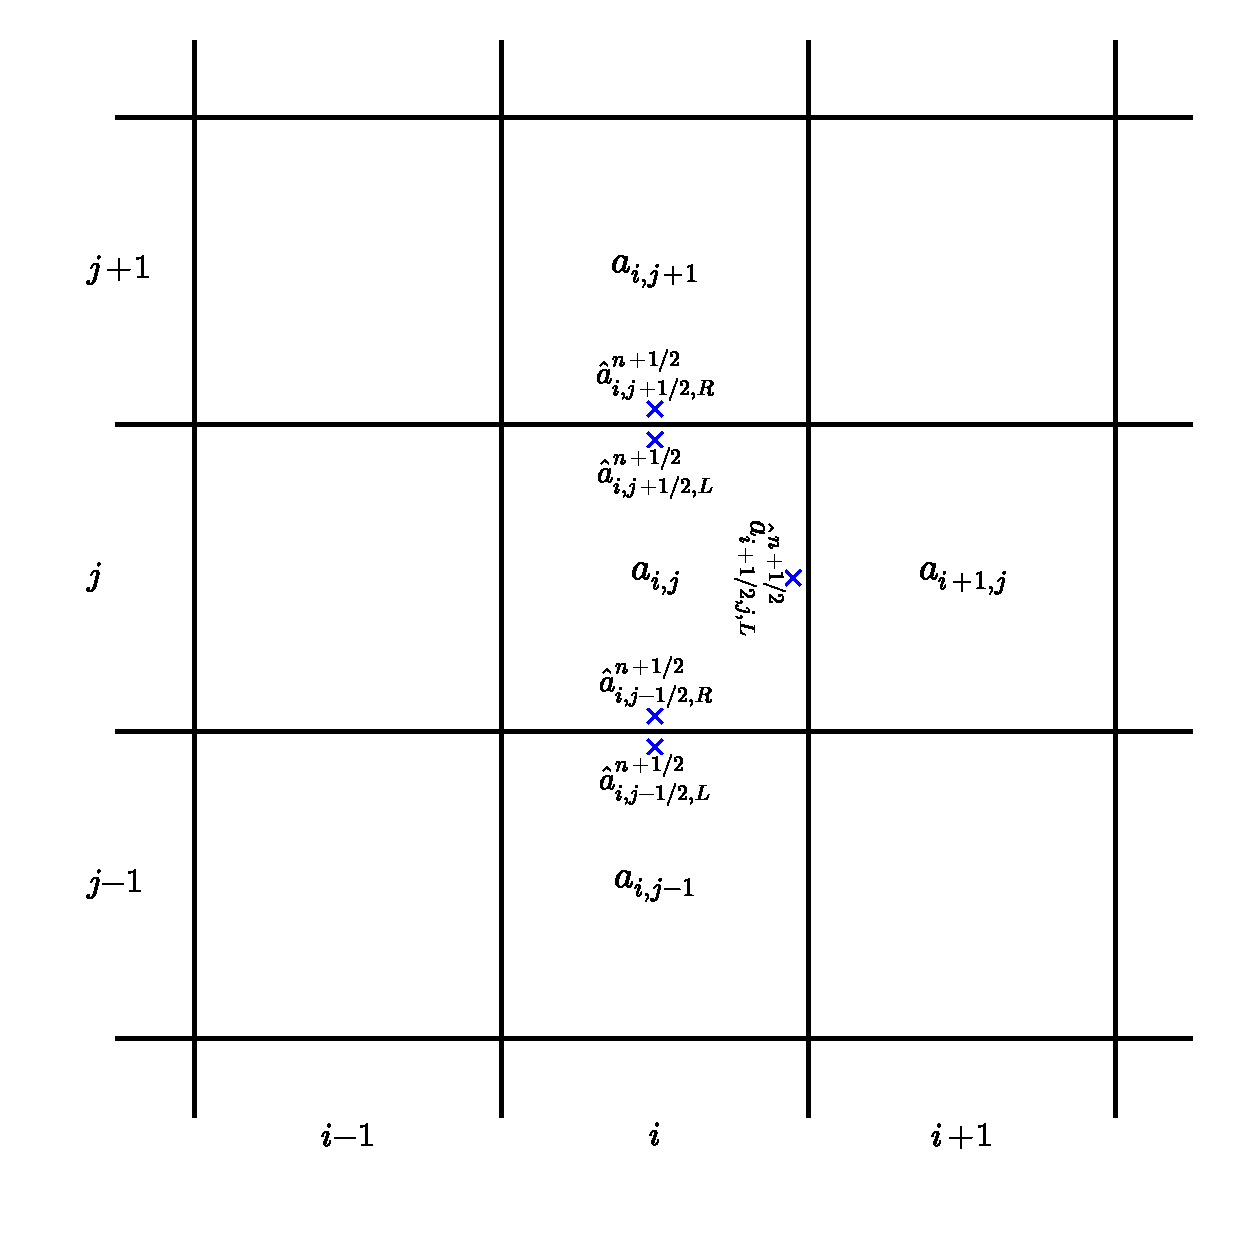
\includegraphics[width=3.3in]{2dgrid-hat}
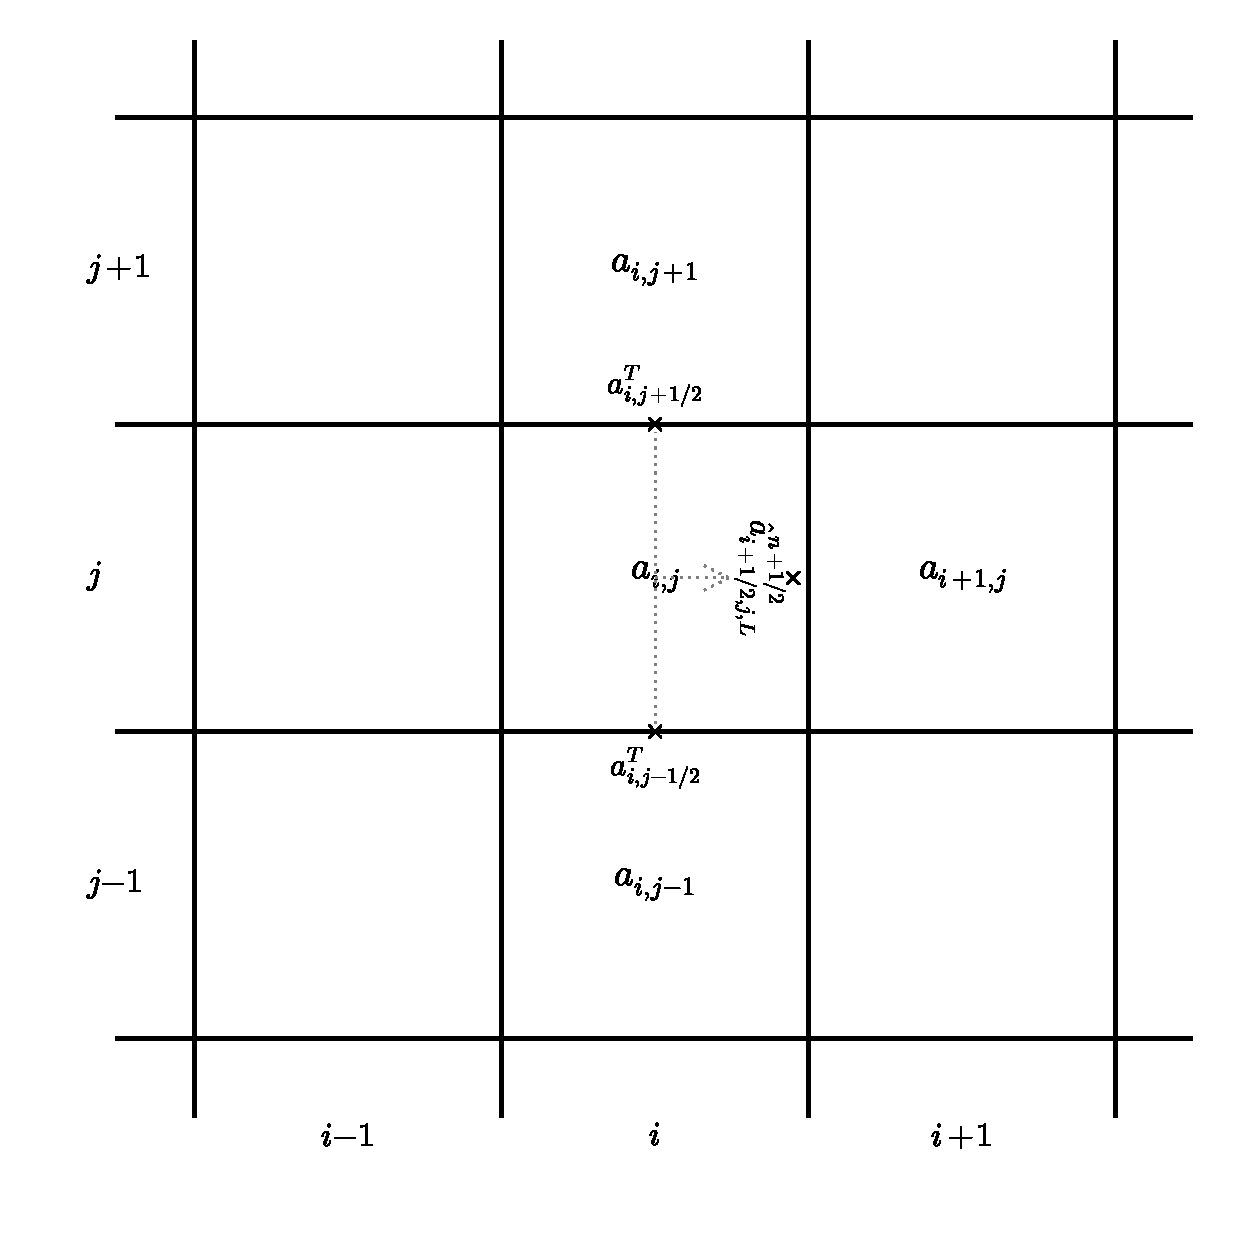
\includegraphics[width=3.3in]{2dgrid-transverse}
\caption{\label{fig:unsplitstates} The construction of the
  $a_{i+1/2,j,L}^{n+1/2}$ state.  Left: first we compute the
  $\hat{a}$'s---here we show all of the $\hat{a}$'s that will be used
  in computing the full left interface state at $(i+1/2,j)$.  Right:
  after the transverse Riemann solves, we have the two transverse
  states ($a^T_{i,j+1/2}$ and $a^T_{i,j-1/2}$) that will be
  differenced and used to correct $\hat{a}_{i+1/2,j,L}^{n+1/2}$
  (illustrated by the dotted lines) to make $a_{i+1/2,j,L}^{n+1/2}$.}
\end{figure}

Once all of the full states (normal prediction $+$ transverse flux
difference) are computed to the left and right of all the interfaces
($x$ and $y$), we solve another Riemann problem to find the final 
state on each interface.
\begin{equation}
a_{i+1/2,j}^{n+1/2} = \mathcal{R}(a_{i+1/2,j,L}^{n+1/2},
                                  a_{i+1/2,j,R}^{n+1/2}) \\
\end{equation}
The final conservative update is then done via Eq.~\ref{eq:update2du}.

See \cite{colella:1990} for more details on this unsplit method.


\section{Burger's equation}

The inviscid Burger's equation is the simplest nonlinear hyperbolic
equation:
\begin{equation}
u_t + u u_x = 0
\end{equation}
Here $u$ is both the quantity being advected and the speed at which 
it is moving.
In conservative form, this appears as:
\begin{equation}
u_t = \left [\tfrac{1}{2} u^2 \right ]_x = 0
\end{equation}

The solution of this follows the same methodology as outlined above.

The Riemann problem differs from linear advection.  It remains the
case that the solution is constant along the lines $x = ut + x_0$ (the
characteristics), but now those lines are no longer parallel.  If the
characteristic lines intersect, then there it is not possible to trace
backward from time to learn where the flow originated.  This is the 
condition for a {\em shock}.

Shock speed from jump conditions

Riemann problem
\begin{eqnarray}
\mathrm{if~} u_l > u_r:&& u_s = \left \{ \begin{array}{cl}
                u_l & \mathrm{if~} S > 0 \\ 
                u_r & \mathrm{if~} S < 0 \\
                0   & \mathrm{if~} S = 0 \end{array} \right . \\[1em]
\mathrm{otherwise:}&& u_s = \left \{ \begin{array}{cl}
                u_l & \mathrm{if~} u_l \ge 0 \\  
                u_r & \mathrm{if~} u_l \le 0 \\  
                0   & \mathrm{otherwise} \end{array} \right .
\end{eqnarray}
               

\begin{figure}
\centering
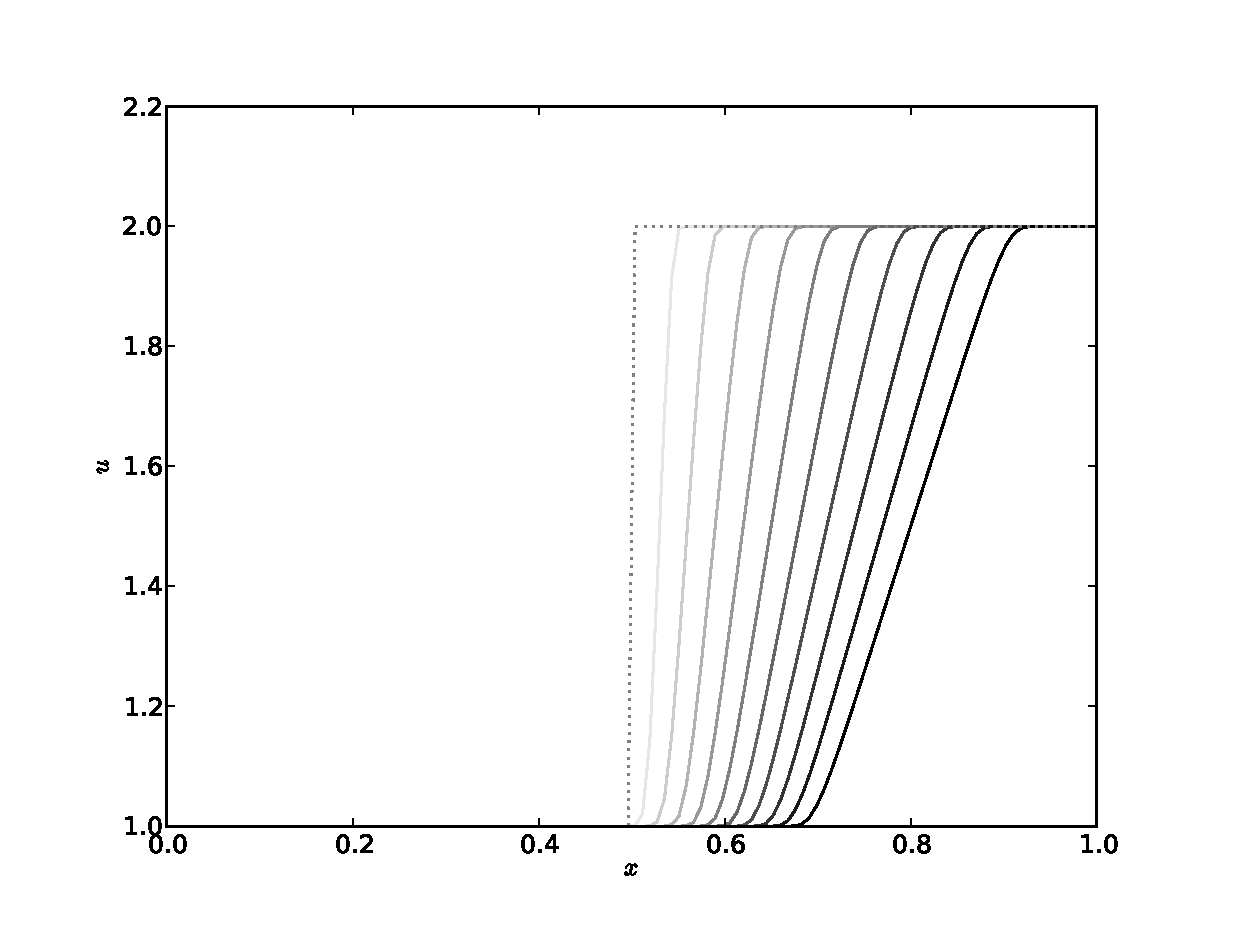
\includegraphics[width=3.25in]{fv-burger-rarefaction}
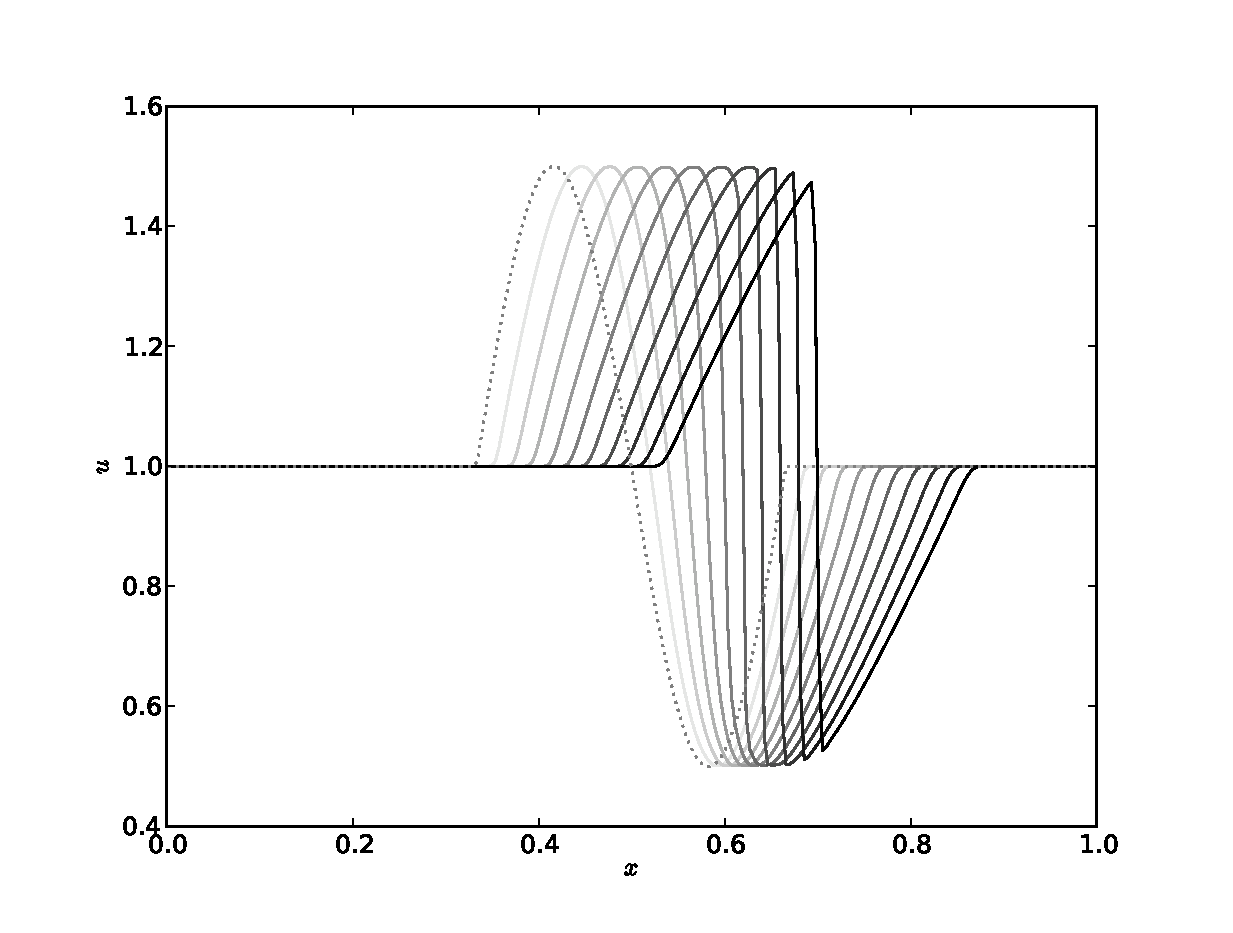
\includegraphics[width=3.25in]{fv-burger-sine}
\end{figure}

\section{Going further}

\begin{itemize}
\item {\em Stability analysis}: many texts provide the details of von
  Neumann stability analysis for the linear advection equation.
  There, you will see how a Fourier analysis can be used to derive the
  CFL condition.  Note: this stability analysis is restricted to
  linear equations, but we nevertheless use the resulting limits for
  nonlinear equations (like the Euler equations).

\item {\em Slope limiting}: there are a wide variety of slope limiters.
  All of them are designed to reduce oscillations in the presence
  of discontinuties or extrema, but some are higher-order and can be
  less restrictive when dealing with smooth flows.  Most hydro
  texts (e.g.\ \cite{leveque:2002,toro:1997}) provide an introduction to the design
  of such limiters.

\item {\em Multi-dimensional limiting}: the procedure described above
  still does the limiting in each dimension indepedent of the other
  when doing the unsplit reconstruction.  This can lead to overshoots/
  undershoots.  An example of a method that considers the limiting
  in multidimensions is \cite{BDS,quadBDS}.

\end{itemize}


\bibliographystyle{plain}
\bibliography{refs}

\end{document}
